\documentclass[t,usepdftitle=false]{beamer}

\usepackage[utf8]{inputenc}
\usetheme{Singapore}
\usepackage{xcolor}
\setbeamertemplate{footline}[frame number]

\usepackage{etex}
\usepackage{pictex}
\usepackage{tikz}
\usetikzlibrary{shapes,arrows}
\usepackage{pgfplots}

\usepackage{amsmath}

% \setbeamercovered{transparent}
%\usecolortheme{crane}
\title[Simulation]{Discrete event simulation}

\author[Fabian Bastin]{Fabian Bastin \\ \url{fabian.bastin@umontreal.ca} \\ Université de Montréal -- CIRRELT -- IVADO -- Fin-ML}
\date{}

\def\bu{\boldsymbol{u}}
\def\bU{\boldsymbol{U}}
\def\cS{\mathcal{S}}

\begin{document}
\frame{\titlepage}

% ------------------------------------------------------------------------------------------------------------------------------------------------------
\begin{frame}
	\frametitle{Basic concepts}
	
	\begin{description}
		\item[System]
		collection d'entités qui agissent et interagissent afin d'accomplir une certaine fin logique.\\
		L'état d'un système est la collection de variables nécessaires pour décrire un système à un instant particulier.
		\item[Model]
		description simplifiée d'un système, dans le but d'évaluer sa performance ou l'effet de certaines décisions.
		\item[Simulation]
		faire évoluer le modèle d'un système en fournissant les entrées appropriées, puis observer et analyser les résultats.
	\end{description}
	
	\mbox{}
	
	Two main system types: discrete and continuous.Deux types principaux de systèmes: discrets et continus.
	
\end{frame}

\begin{frame}
	\frametitle{Models}
	
	Physical vs mathematical model.
	
	\mbox{}
	
	Analytical model, numerical model, model with simulation.

\mbox{}

Reference textbook: 
A. M. Law, Simulation Modeling and Analysis, fifth edition, McGraw-Hill, USA, 2015.

\end{frame}

\begin{frame}
\frametitle{Event approach}

Assumption: system in which state variables can only change by a countable number of points in time.

\mbox{}

Sequence of events $e_0, e_1, e_2\ldots$, occurring at times $0 \leq t_0 \leq t_1 \leq t_2 \leq \ldots$. 

\mbox{}

${\cS_i}$: system state immediately after ${e_i}$.

\mbox{}

simulation time: current value of ${t_i}$.

\mbox{}

$(t_i,\cS_i)$ must contain enough information to continue the simulation (except the realizations of the random variables for events $e_j$, $j > i$).

\end{frame}

\begin{frame}
\frametitle{Discrete events}

\begin{center}
%%  Evolution of a general discrete-event model.
\hspace{0.5cm}
\beginpicture
\setcoordinatesystem units <7pt,7pt>
%%  72.27pt = 1in
\setplotarea x from 0 to 36, y from 0 to 10
\axis left
  label {\lines {\emph{state}\cr\vbox to 95pt{\hbox to 1.5pt{\null }} \cr}
         \hskip 9pt } /

\axis bottom
  label {\hbox to 4.0in {\hfill \emph{time}}}
  ticks length <4pt> withvalues 
     0 $t_1$ $t_2$ $t_3$ $t_4$ $t_5$ $t_6$ /
  at 0.0 6.0 7.5 12.5 18.0 25.2 30.0 / /

\axis bottom /
\put {$\rightarrow$} at 36.0 -0.1 
\put {$\uparrow$}    at 0.0 10.0 
\multiput {$\bullet$} at
  0.0 2.0
  6.0 1.6
  7.5 2.7
 12.5 6.1
 18.0 5.1
 25.2 2.6
 30.0 4.0 /
\putrule from  0.0 2.0 to  6.0 2.0
\putrule from  6.0 1.6 to  7.5 1.6
\putrule from  7.5 2.7 to 12.5 2.7
\putrule from 12.5 6.1 to 18.0 6.1
\putrule from 18.0 5.1 to 25.2 5.1
\putrule from 25.2 2.6 to 30.0 2.6
\putrule from 30.0 4.0 to 32.0 4.0 
\endpicture
\end{center}

\end{frame}

\begin{frame}
\frametitle{General framework}

\begin{itemize}
\item
Main program.
\item
Simulation clock.
\item
Event list.
\item
Random numbers generation functions.
\item
Statistical collectors.
\item
Report generation.
\end{itemize}

Event: action, schedule, cancel.

\end{frame}

\begin{frame}

\tikzstyle{decision} = [diamond, draw, fill=blue!20,
    text width=2.5cm, text badly centered, node distance=1cm, inner sep=0pt]
\tikzstyle{block} = [rectangle, draw, fill=blue!20,
    text width=2.5cm, text centered, rounded corners, minimum height=4em]
\tikzstyle{line} = [draw, very thick, color=black!50, -latex']
\tikzstyle{cloud} = [draw, ellipse,fill=yellow!20, node distance=1cm,
    minimum height=2em]

\begin{footnotesize}
\begin{center}
\begin{tikzpicture}[scale=0.09, node distance = 0.8cm, auto]
    % Place nodes
    \node [block] (init) {Initialization};
    \node [text width=2.2cm, cloud, left of=init, node distance=3.7cm] (clock) {Set simulation clock to 0};
    \node [text width=2.5cm, cloud, right of=init, node distance=3.7cm] (system) {Plan first event(s)};
    \node [text width=2.1cm, cloud, below of=init, node distance=2.0cm] (premier) {Pull the first event};
    \node [text width=2.1cm, block, below of=premier, node distance=2.0cm] (event) {Handle current event};
    \node [text width=2.1cm, block, below of=event, node distance=2.0cm] (schedule) {Plan resulting events};
    \node [block, left of=schedule, node distance=4.0cm] (update) {Pull next event and advance clock};
    \node [text width=2.1cm, decision, below of=schedule, node distance=4.0cm] (decide) {Liste d'événements vide ou événement de fin?};
    \node [block, below of=decide, node distance=4.5cm] (stop) {Stop};
    % Draw edges
    \path [line] (init) -- (premier);
    \path [line] (premier) -- (event);
    \path [line] (event) -- (schedule);
    \path [line] (schedule) -- (decide);
    \path [line] (decide) -| node [near start, color=black] {non} (update);
    \path [line] (update) |- (event);
    \path [line] (decide) -- node [, color=black] {oui}(stop);
    \path [line,dashed] (clock) -- (init);
    \path [line,dashed] (system) -- (init);
\end{tikzpicture}
\end{center}
\end{footnotesize}

\end{frame}

\begin{frame}

\tikzstyle{decision} = [diamond, draw, fill=blue!20,
    text width=2.5cm, text badly centered, node distance=2.5cm, inner sep=0pt]
\tikzstyle{block} = [rectangle, draw, fill=blue!20,
    text width=2.5cm, text centered, rounded corners, minimum height=4em]
\tikzstyle{line} = [draw, very thick, color=black!50, -latex']
\tikzstyle{cloud} = [draw, ellipse,fill=yellow!20, node distance=2.5cm,
    minimum height=2em]

\begin{footnotesize}
\begin{center}
\begin{tikzpicture}[scale=0.09, node distance = 1cm, auto]
    % Place nodes
    \node [text width=3cm, block, below of=premier, node distance=2cm] (event) {Handle current event};
    \node [text width=3cm, block, below of=event, node distance=2cm] (schedule) {Plan resulting events};
    \node [block, left of=schedule, node distance=4.5cm] (update) {Pull next event and advance clock};
    \node [text width=1.9cm, decision, below of=schedule, node distance=2.5cm] (decide) {End event or empty event list?};
    \node [block, below of=decide, node distance=2.5cm] (stop) {Stop and print report};
    % Draw edges
    \path [line] (event) -- (schedule);
    \path [line] (schedule) -- (decide);
    \path [line] (decide) -| node [near start, color=black] {no} (update);
    \path [line] (update) |- (event);
    \path [line] (decide) -- node [, color=black] {yes}(stop);
\end{tikzpicture}
\end{center}
\end{footnotesize}

\end{frame}

\begin{frame}
\frametitle{Queueing systems}

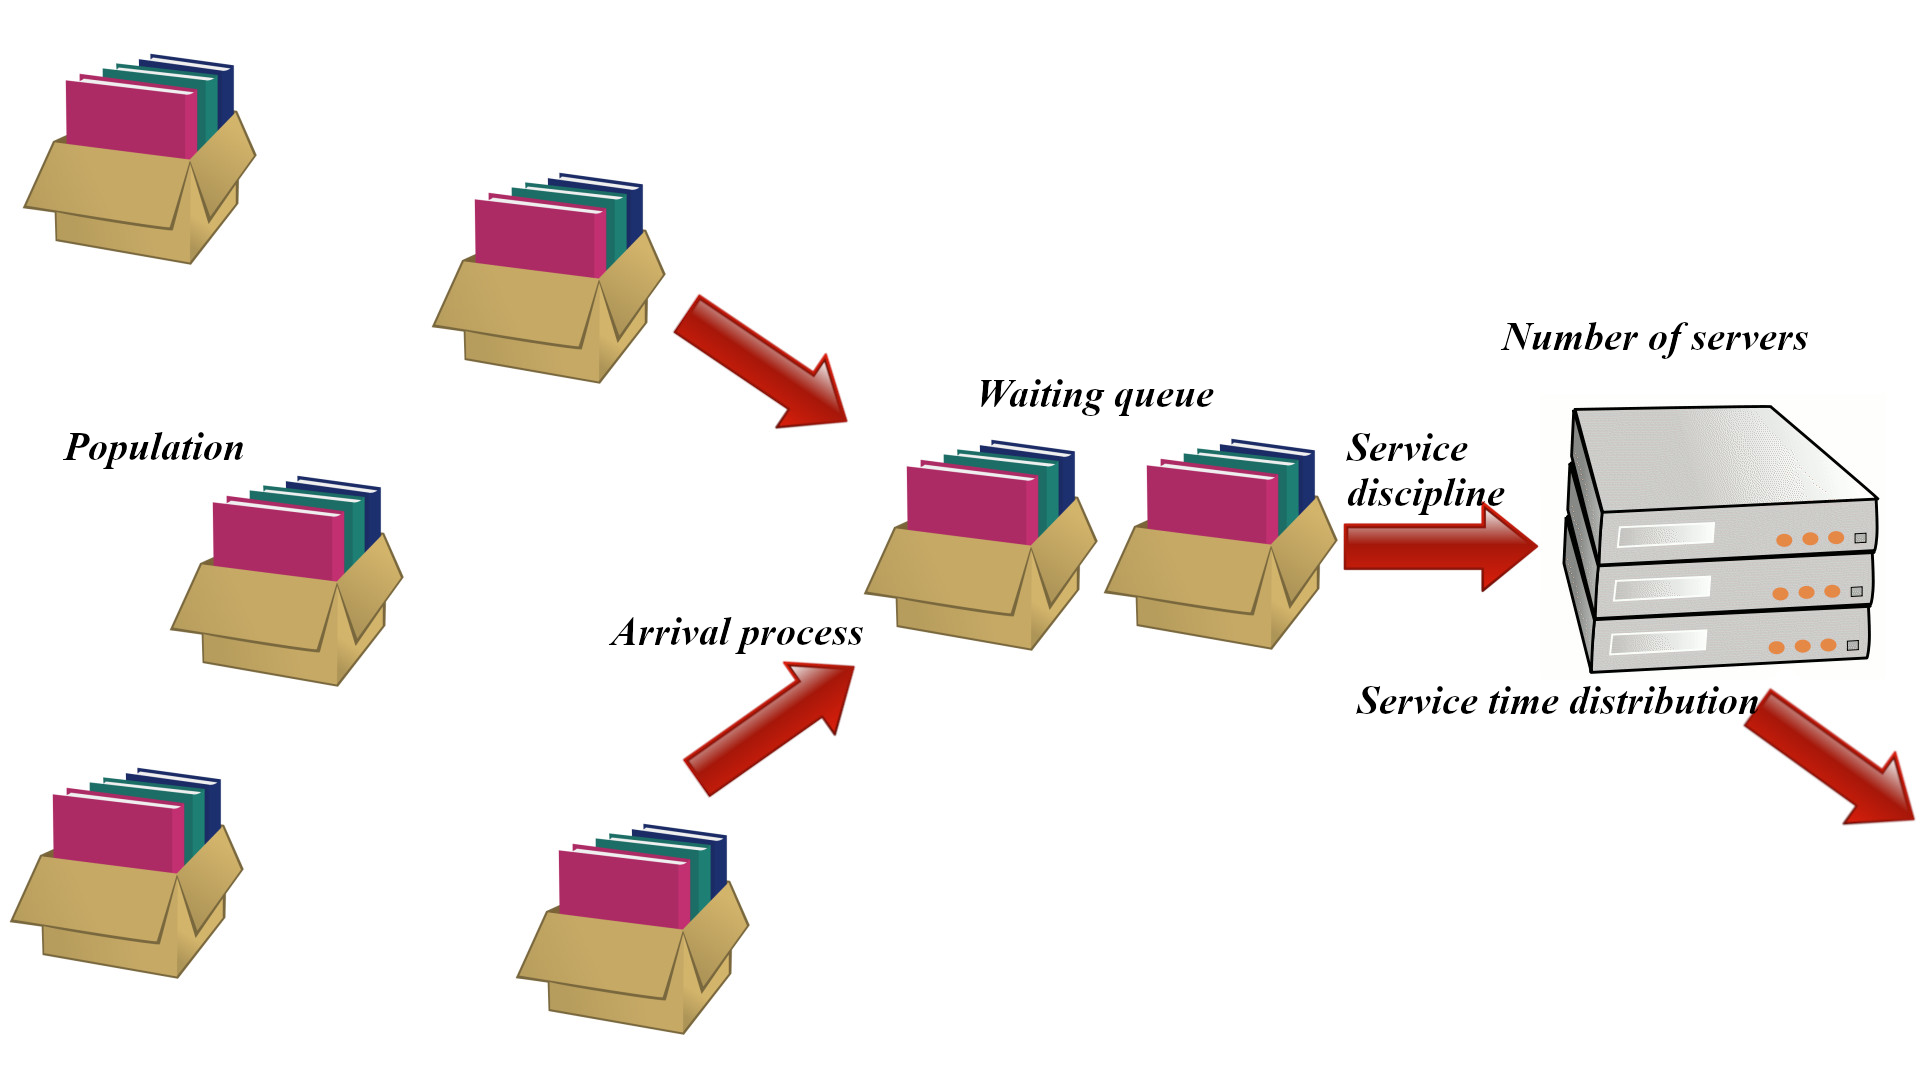
\includegraphics[width=\textwidth]{imgs/queue-labels.png}

\end{frame}

\begin{frame}
\frametitle{Kendall notation}

$$
A/S/c/K/N/SD
$$

\mbox{}

\begin{description}
	\item[$A$]
Arrival process
	\item[$S$]
Service time distribution
	\item[$c$]
Number of servers
	\item[$K$]
Waiting list maximum length
	\item[$N$]
Population size
	\item[$SD$]
Service discipline
\end{description}
 
\end{frame}

\begin{frame}
\frametitle{Notation}

\begin{description}
	\item[$G$]
	General
	\item[$I$]
	Independent
	\item[$M$]
	Markovian or memoryless
\end{description}

\mbox{}

Defaults:
\begin{itemize}
	\item
	Infinite buffer capacity
	\item
	Infinite population size
	\item
	FCFS (First-Come-First-Served) service discipline
\end{itemize}

\mbox{}

Memoryless property:
$$
P[X > x +a \,|\, X > a] = P[X > x]
$$
Continuous: exponential distribution\\
Discrete: geometric distribution 

\end{frame}

\begin{frame}
\frametitle{Example: GI/G/1 queue}

$$
G/G/1 = G/G/1/\infty/\infty/FCFS
$$

We also write $GI/G/1$ to stress that the service times are independent.

\mbox{}

The clients arrive one by one, one being served at a time, under a FCFS priority, with
\begin{itemize}
\item
${S_i}$: service time of client $i$, with cdf $G$;
\item
${A_i}$: inter-arrival time between clients $i$ and $i+1$, with cdf $F$.
\end{itemize}
We assume $S_i$ and $A_i$ mutually independent.

\end{frame}

\begin{frame}
\frametitle{Example: GI/G/1 queue}

The first client arrives at time ${A_0}$ in an empty system.

\mbox{}

Nous souhaitons simuler ce système pour une durée ${T}$ et calculer
l'attente moyenne par client et la longueur moyenne de la file d'attente.
Les types d'événements sont
\begin{enumerate}
\item
arrivée;
\item
départ;
\item
fin de la simulation.
\end{enumerate}
Les variables aléatoires (indépendentes) à générer sont $A_1, A_2,
A_3, \dots$ et $S_1, S_2, S_3, \dots$.

\end{frame}

\begin{frame}
\frametitle{Example: GI/G/1 queue}

\begin{itemize}
\item
${W_i}$, le temps d'attente du client $i$;
\item
${Q(t)}$, la longueur de la file d'attente au temps $t$;
\item
${N_c(t)}$, le nombre de clients ayant débuté leur service durant l'intervalle $[0,t]$.
\end{itemize}
Supposons que nous voulons calculer, pour l'intervalle $[0,T]$,
l'\emph{attente moyenne} par client,
\[
 {\overline{W}_{N_c(T)}} = {1\over N_c(T)} \sum_{i=1}^{N_c(T)} W_i;
\]
et la \emph{longueur moyenne} de la file d'attente:
\[
 {\overline{Q}_T} = {1\over T} \int_0^T Q(t) dt.
\]

\end{frame}

\begin{frame}
\frametitle{Example: GI/G/1 queue}

Cette dernière intégrale est facile à calculer par simulation.

\mbox{}

Pour chaque \emph{client}, nous créons un \emph{objet} contenant l'instant  d'arrivée et la durée de service.

\mbox{}

Variables d'état: liste des clients en attente et la liste les clients en service.

\mbox{}

+ horloge de simulation,
compteurs statistiques (au besoin), \emph{liste} des événements futurs prévus, 
 par ordre chronologique, et une procédure pour chaque type d'événement.
 
\end{frame}

\begin{frame}
\frametitle{Queueing system simulation}

\begin{small}
\begin{description}
\item[Arrivée]
Générer $A$ selon $F$ et prévoir une autre arrivée 
    dans $A$ unités de temps;\\
Créer le nouveau client et noter son instant d'arrivée;\\
Générer sa durée de service $S$ selon $G$;\\
{\bf Si} (serveur est occupé) {\bf alors}\\
\quad Insérer ce client dans la liste des clients en attente;\\
{\bf sinon}\\
\quad   Insérer le client dans la liste des clients en service;\\
\quad   Prévoir son départ dans $S$ unités de temps; \\
Mise à jour des statistiques voulues.
\item[Départ]
Enlever le client de la liste des clients en service;\\
{\bf Si} la file d'attente n'est pas vide {\bf alors}\\
\quad  Enlever le premier client de la liste d'attente;\\
\quad  L'insérer dans la liste des clients en service;\\
\quad  Récupérer son $S$ et prévoir son départ dans 
       $S$ unités de temps;\\
Mise à jour des statistiques voulues.
\item[Fin-de-la-Simulation]
Imprimer un rapport et terminer le programme.
\end{description}
\end{small}
\end{frame}

\begin{frame}
\frametitle{Simulation}

Démarrer la simulation:
\begin{itemize}
\item
initialiser des variables et compteurs,
\item
prévoir la ``Fin-de-la-Simulation'' au temps $T$
\item
générer $A$ selon $F$ et prévoir la première ``Arrivée'' dans $A$ unités de temps,
\item
lancement de la simulation.
\end{itemize}

\mbox{}

L'exécution de la simulation consiste simplement à répéter la boucle
suivante:\\
{\bf Répéter:} exécuter le prochain événement
     dans la liste d'événements\\
{\bf jusqu'à:} la liste des événements prévus est vide,\\
\quad    ou bien un événement stoppe la simulation.

\end{frame}

\begin{frame}
\frametitle{Simulation sans liste d'événements.}

Pas toujours indispensable de recourir à l'approche par événements.

\mbox{}

Exemple: récurrence de Lindley:
\[
 W_1 = 0,\quad W_{i+1} = \max(0,\; W_i + S_i - A_{i+1}).
\]

Nous pouvons ainsi facilement simuler pour un nombre fixe de clients (au lieu d'un horizon de temps $T$ fixe).

\mbox{}

Le formulation du programme basée sur la récurrence de Lindsley revient à traiter un problème d'intégration sur $[0,1)^t$.

\end{frame}

\begin{frame}
\frametitle{Récurrence de Lindley}

Supposons que nous souhaitions estimer $E[\overline{W}_{100}]$ par
${\overline{W}_{100}}$:
\[
{\overline{W}_{100}} = \frac{1}{100} \sum_{i=1}^{100} W_i.
\]

\mbox{}

Il nous faut $A_1, S_1, A_2, S_2, \dots, A_{99}, S_{99}$.
Si on pose ${A_i} = F^{-1}(U_{2i-1})$ et ${S_i} = G^{-1}(U_{2i})$, où
$U_j$, $j = 1,\ldots,99$, sont des variables aléatoires uniformes sur
$(0,1)$, alors $\overline{W}_{100} = f(U_1,\dots,U_{198})$ ($f$ étant de
forme inconnue dans le cas présent).

\mbox{}

Nous avons donc $t=198$, i.e., 
\[
  E[\overline{W}_{100}] = \int_{[0,1)^{198}} f(\bu)d\bu.
\]

\end{frame}

\begin{frame}
\frametitle{Nombre aléatoire de clients}

Par contre, si nous voulons simuler $\overline{W}_{N_c(T)}$, le nombre de clients
$N_c(T)$ est aléatoire et non borné.
Nous devrions donc choisir $t=\infty$ comme dimension.

\end{frame}

\begin{frame}
\frametitle{Approche par processus}

Un processus est une séquence temporellement ordonnée d'événements interreliés, séparés par certains intervalles de temps,
qui décrit l'expérience entière d'une ``entité'' comme celle-ci évolue à travers un ``système''.
Un système ou un modèle de simulation peut avoir différents types de
processus.

\mbox{}

Une routine sera associée à chaque processus du modèle, décrivant son
histoire entière à travers le système.

\mbox{}

Au contraire de l'approche par événements, une routine de processus
contient explicitement le passage du temps simulé et a généralement de
multiples points d'entrée.

\end{frame}

\begin{frame}
\frametitle{Processes vs Events}

Une simulation utilisant l'approche par processus évolue aussi au
cours du temps en exécutant les événements dans l'ordre de leur
occurence.

\mbox{}

En interne, les approches par événement et par processus sont donc
très similaires.

\mbox{}

Pour l'utilisateur, le raisonnement soit
différent, et puisse parfois (mais pas toujours) être plus naturel pour l'approche par processus.

%\mbox{}

%En outre, l'approche par processus est souvent plus lente en terme de
%temps d'exécution, puisque le simulateur doit au final traiter des
%événements, et gérer des processus pouvant être concurrents.

\end{frame}

\begin{frame}
	\frametitle{Amélioration de l'Efficacité}

The following material is adapted from Pierre L'Ecuyer's class ``Simulation: stochastic aspects''..

\mbox{}
	
	L'efficacité d'un estimateur $X$ se
	définit comme suit:
	$$
	eff[X] = {1\over MSE[X] C(X)},
	$$
	where MSE stands for mean square error and $C(X)$ represents the cost to compute $X$.
	
	\mbox{}
	
	Est-il possible, étant donné $X$, de construire un nouvel estimateur $Y$ plus efficace que $X$?
	
	\mbox{}
	
	Nous allons introduire les principaux concepts d'amélioration de l'efficacité au moyen d'un exemple introductif sur les centres d'appels téléphoniques.
	
\end{frame}

\begin{frame}
	\frametitle{Exemple introductif}
	
	Posons ${B}$, le \emph{facteur d'achalandage} pour la journée, et
	supposons que $P[B = b_t] = q_t$, o\`u
	\begin{center}
		\begin{tabular}{c|cccc}
			${t}$   &   1  &  2   &   3  &  4  \\  
			\hline
			${b_t}$ &  0.8 &  1.0 &  1.2 &  1.4 \\
			${q_t}$ & 0.25 & 0.55 & 0.15 & 0.05 \\
		\end{tabular}
	\end{center}
	
	\mbox{}
	
	Il est facile de vérifier que $E[B] = 1$. %% et $\Var[B] = 0.024$.
	
	\mbox{}
	
	Les \emph{arrivées} des appels suivent processus de Poisson de taux
	$B{\lambda_j}$ durant l'heure $j$.
	
	\mbox{}
	
	Notons ${G_i(s)}=$ nombre d'appels dont le service a débuté
	après moins de ${s}$ secondes d'attente, le jour $i$.
	
	\mbox{}
	
	On veut estimer ${\mu} = E[G_i(s)]$, disons pour ${s=20}$.
	
\end{frame}

\begin{frame}
	\frametitle{Example}
	
	Nous supposons de plus que les durées de service des appels suivent la loi
	$\Gamma(\alpha,\gamma)$, dont la moyenne est $\alpha\gamma$.
	
	\mbox{}
	
	Dans notre exemple, on a $\alpha = 1$ et $\gamma = {\gamma_1} = 100$.
	
	\mbox{}
	
	Nombre d'agents $n_j$ et taux d'arrivée $\lambda_j$ (par heure) pour 13 périodes d'une heure dans le centre d'appel:
	
	\begin{footnotesize}
		\hspace*{-1cm}
		\begin{tabular}{l|rrrrrrrrrrrrr}
			\hline
			$j$   & 0 & 1 & 2 & 3 & 4 & 5 & 6 & 7 & 8 & 9 & 10 & 11 & 12 \\
			$n_j$ & 4 & 6 & 8 & 8 & 8 & 7 & 8 & 8 & 6 &  6 &  4 &  4 &  4 \\
			$\lambda_j$ & 100 & 150 & 150 & 180 & 200 & 150 & 150 & 150 & 
			120 & 100 & 80 & 70 & 60 \\
			\hline
		\end{tabular}
	\end{footnotesize}
	
	\mbox{}
	
	We simulate ${n}$ independent days.
	
\end{frame}

\begin{frame}
	\frametitle{Example}
	
	Soit ${X_i} = G_i(s)$ pour le jour $i$, et 
	\[
	{\bar X_n} = {1\over n} \sum_{i=1}^n X_i.
	\]
	On a $E[\bar X_n] = \mu$ et $Var[\bar X_n] = Var[X_i]/n$.
	
	\mbox{}
	
	Une expérience avec ${n = 1000}$ donne $\bar X_n = 1518.3$ et $S_n^2
	= {21615}$.
	La variance estimée de $\bar X_n$ est alors $\widehat{Var}[\bar X_n] = 21.6$.
	
\end{frame}

\begin{frame}
	\frametitle{Exemple introductif}
	
	Nous souhaitons construire un intervalle de confiance pour $\sigma^2 = n Var[\bar X_n]$, sous
	l'hypothèse que $(n-1)S_n^2/\sigma^2$ suit approximativement une $\chi^2$ à ${n-1}$ degrés de
	liberté. Ceci permet de construire l'intervalle à $90\%$: $[0.930S_n^2, 1.077S_n^2]$.
	
	\mbox{}
	
	En d'autres termes, l'erreur relative de cet estimateur est inférieure \`a $8\%$ avec une
	``confiance'' d'environ 90\%.
	
	\mbox{}
	
	Voyons comment \emph{améliorer} cet estimateur $\bar X_n$,
	en réduisant sa variance. Pour chaque méthode proposée, 
	nous donnerons des résultats numériques pour {$n = 1000$}.
	
\end{frame}

\begin{frame}
	\frametitle{Estimation indirecte.}
	
	Soit ${A_i}$ le nombre total d'arrivées au jour $i$; posons ${D_i} = A_i - X_i$.
	
	\mbox{}
	
	On sait que ${a} = E[A_i] = \sum_{j=1}^m \lambda_j = 1660$.
	
	\mbox{}
	
	Nous pouvons dès lors écrire $\mu = E[X_i] = E[A_i - D_i] = a - E[D_i]$, que 
	l'on peut estimer par
	$$ {\bar X_{\rm{i},n}} = E[A_i] - \bar D_n = a - {1\over n} \sum_{i=1}^n D_i.$$
	
	\mbox{}
	
	Cet estimateur a moins de variance que $\bar X_n$ ssi $Var[D_i] < Var[X_i]$. 
	Variance estimée: $\widehat{Var}[X_{\rm{i},i}] = {18389}$.
	
\end{frame}

\begin{frame}
	\frametitle{Control variate (CV)}
	
	Idée: exploiter l'information auxiliaire.
	
	\mbox{}
	
	Par exemple, si ${A_i}$ est plus grand que d'habitude ($A_i > E[A_i] = 1660$),
	on s'attend \`a ce que ce jour l\`a, $X_i$ et $D_i$
	\emph{surestiment} $E[X_i]$ et $E[D_i]$.
	
	\mbox{}
	
	On pourrait faire une ``\emph{correction}'' \`a ces estimateurs:
	remplacer $X_i$ par
	$$ X_{\rm{c},i} = X_i - {\beta} (A_i - 1660) $$
	o\`u $\beta$ est une constante appropriée.  \ Alors
	\[
	{\bar X_{\rm{c},n}} = \bar X_n - \beta (\bar A_n - 1660).
	\]
	
\end{frame}

\begin{frame}
	\frametitle{Control variate (CV)}
	
	On a $E[\bar X_{\rm{c},n}] = E[X_i]$ et 
	$$ Var[\bar X_{\rm{c},n}] 
	= \frac{Var[X_i] + \beta^2Var[A_i] - 2 \beta Cov[A_i,X_i]}{n}. $$ 
	Cette variance est une fonction quadratique en $\beta$, que l'on minimise
	en prenant
	\[
	\beta = {\beta^*} = Cov[A_i, X_i] / Var[A_i].
	\]
	
	\mbox{}
	
	La \emph{variance minimale} est
	$$ Var[\bar X_{\rm{c},n}] = \frac{Var[X_i] - (\beta^*)^2 Var[A_i]}{n}
	= Var[\bar X_n] (1- \rho^2[A_i,X_i]) $$
	o\`u ${\rho[A_i, X_i]}$ est le coeff.\ de corrélation entre 
	$A_i$ et $X_i$.
	
\end{frame}

\begin{frame}
	\frametitle{Control variate (CV)}
	
	On ne connaît pas $Cov[A_i, X_i]$, mais:
	\begin{enumerate}[(a)]
		\item
		On peut l'estimer par des \emph{expériences pilotes}.
		\item
		On peut l'estimer par les \emph{m\^emes $n$ simulations} que $\bar X_n$.
	\end{enumerate}
	
	\mbox{}
	
	Avec (b) on obtient l'estimateur (légèrement biaisé):
	\[
	\bar X_{\rm{c}e,n} = \bar X_n - {1\over n-1} \left[\sum_{i=1}^n
	(A_i-\bar A_n)(X_i-\bar X_n)\right] {\bar A_n - a\over Var[A_i]}.
	\]
	
	\mbox{}
	
	Conditionnellement \`a $B_i$, $A_i\sim\mbox{Poisson}(1660 B_i)$.  On a donc
	\begin{align*}
		{Var[A_i]} &= Var[E[A_i|B_i]] + E[Var[A_i|B_i]] \\
		&= Var[1660 B_i] + E[1660 B_i] \\
		&= 1660^2 Var[B_i] + 1660 E[B_i] \\
		&= 67794.4.
	\end{align*}
	Variance empirique obtenue ici: {3310}.
	
\end{frame}

\begin{frame}
	\frametitle{Variable de contrôle (VC)}
	
	En prenant $\beta=1$, on retrouve l'estimateur indirect:
	\[
	\bar X_{\rm{i},n} = \bar X_n - (\bar A_n - 1660) = 1660 - \bar D_n.
	\]
	Si on combine \emph{VC + indirect}, on obtient:
	\begin{eqnarray*}
		{\bar X_{\rm{i},\rm{c},n}} &=& a - \bar D_n - \beta_2 (\bar A_n - a) \\
		&=& \bar A_n - \bar D_n -(1+\beta_2)(\bar A_n - a) \\
		&=& \bar X_n -(1+\beta_2)(\bar A_n - a),
	\end{eqnarray*}
	i.e., $\bar X_{\rm{i},\rm{c},n}$ est équivalent \`a $\bar X_{\rm{c},n}$ 
	avec $\beta = 1+\beta_2$.
	Par conséquence, en présence de la variable de contrôle, l'estimation indirecte n'apporte rien.
	
	\mbox{}
	
	Nous pourrions aussi considérer d'autres variables de contrôle, comme $B_i$, la moyenne des durées de service, etc.
	
\end{frame}

\begin{frame}
	\frametitle{Stratification.}
	
	Le facteur d'achalandage ${B_i}$ est une source importante de variabilité 
	importante dans le cas présent. Essayons de la contr\^oler.
	
	\mbox{}
	
	En posant $\mu_t = E[X_i\mid B_i=b_t]$, on a
	\begin{eqnarray*}
		\mu &=& E[X_i]  = \sum_{t=1}^4 P[B_i = b_t]\cdot E[X_i\mid B_i=b_t] \\
		&=&  .25\, E[X_i\mid B_i=0.8] + .55\, E[X_i\mid B_i=1.0]  \\
		&& + .15\, E[X_i\mid B_i=1.2] + .05\, E[X_i\mid B_i=1.4]  \\
		&=&  .25\,\mu_1 + .55\, \mu_2 + .15\, \mu_3 + .05\, \mu_4.
	\end{eqnarray*}
	
	\mbox{}
	
	\emph{Idée}: estimer ${\mu_t}$ \emph{séparément} 
	pour chaque $t$.
	
\end{frame}

\begin{frame}
	\frametitle{Stratification}
	
	Supposons qu'il y a ${N_t}$ jours o\`u $B_i = b_t$ et soient
	${X_{t,1}},\dots, {X_{t,N_t}}$ les valeurs de $X_i$ pour ces jours. 
	
	\mbox{}
	
	On peut estimer $\mu_t = E[X_i\mid B_i=b_t]$ par
	$$ {\hat\mu_t} = {1\over N_t} \sum_{i=1}^{N_t} X_{t,i} $$
	et $\mu$ par
	\[
	{\bar X_{\rm{s},n}} = \sum_{t=1}^4 q_t \hat\mu_t.
	= .25 \hat\mu_1 + .55 \hat\mu_2 + .15 \hat\mu_3 + .05 \hat\mu_4.
	\]
	
\end{frame}

\begin{frame}
	\frametitle{Stratification}
	
	On a 
	\begin{align*}
		&  Var[\bar X_{\rm{s},n} \mid N_1, N_2, N_3, N_4] \\
		&= \sum_{t=1}^4 q_t^2 Var[\hat\mu_t | N_t]  
		= \sum_{t=1}^4 q_t^2 \sigma^2_t/N_t \\
		&= .25^2 \sigma^2_1/N_1 + .55^2 \sigma^2_2/N_2 + 
		.15^2 \sigma^2_3/N_3 + .05^2 \sigma^2_4/N_4.
	\end{align*}
	o\`u ${\sigma^2_t} = Var[X_i\mid B_i=b_t]$.
	
	\mbox{}
	
	La variance est réduite si les $\sigma_t^2$ sont inférieurs \`a $Var[X_i]$.
	
	\mbox{}
	
	Si les $B_i$ sont générés normalement: \emph{post-stratification}.
	
	\mbox{}
	
	Pour estimer $\mu$ par stratification, on peut aussi 
	\emph{fixer les $N_t = n_t$ \`a l'avance}, c'est-\`a-dire choisir \`a
	l'avance combien de jours on aura $B_i = b_t$ pour chaque valeur de
	$t$.
	
\end{frame}

\begin{frame}
	\frametitle{Stratification}
	
	\begin{itemize}
		\item
		\emph{Allocation proportionnelle}: prendre ${n_t} = n q_t$.\\
		Avec $n=1000$, cela donne $n_1 = 250$, $n_2 = 550$, $n_3 = 150$, $n_4
		= 50$.
		\item
		\emph{Allocation optimale}: 
		choisir les $n_t$ pour minimiser $Var[\bar X_{\rm{s},n}]$ sous la contrainte
		$n_1+n_2+n_3+n_4=n$.  On obtient:
		\[
		\frac{{n_t}}{n} 
		= {\sigma_t P[B_i=t] \over\sum_{k=1}^4 \sigma_k P[B_i=k]}
		= {\sigma_k q_k \over\sum_{k=1}^4 \sigma_k q_k}.
		\]
		On ne connait pas ces $\sigma_k$, mais on peut les estimer par des 
		essais pilotes.
		Avec ${n_0=800}$ essais pilotes, 200 par valeur de $t$, on obtient par
		exemple $(n_1, n_2, n_3, n_4) = (219, 512, 182, 87)$ (après arrondi). 
	\end{itemize}
	
\end{frame}

\begin{frame}
	\frametitle{Stratégies combinées.}
	
	\emph{Stratification combinée avec VC:}\\
	$$ 
	{\hat\mu_t} = {1\over n_t} \sum_{i=1}^{n_t} X_{\rm{c},t,i} 
	= {1\over n_t} \sum_{i=1}^{n_t} 
	[X_{t,i} - \beta_t (A_{t,i} - a\,b_t)].
	$$
	
	\mbox{}
	
	On minimise ${\sigma_t^2} = Var[X_{\rm{c},t,i}]$ en prenant 
	\[
	\beta_t = {\beta_t^*} = Cov[A_{t,i},\, X_{t,i}] / Var[A_{t,i}]
	= Cov[A_i, X_i | B_i=b_t] / (a b_t).
	\]
	
	\mbox{}
	
	L'ajout d'une VC change les $\sigma_t^2$: l'allocation 
	optimale n'est plus la m\^eme.
	
	\mbox{}
	
	Avec $n_0=800$ essais pilotes, on obtient
	$(\beta_1,\beta_2, \beta_3, \beta_4) = (1.020, 0.648, 0.224, -0.202)$ 
	et $(n_1, n_2, n_3, n_4) = (131, 503, 247, 119)$ 
	comme estimation des valeurs optimales.
	
\end{frame}

\begin{frame}
	\frametitle{Stratégies combinées.}
	
	En répétant l'expérience avec ${n = 100000}$, on peut trouver les
	estimations suivantes pour la variance ($\pm 1\%$):\\
	$Var[X_{n}] = 21998$; \
	$Var[X_{\rm{i},n}] = 17996$; \
	$Var[X_{\rm{c},n}] = 3043$; \
	$Var[X_{\rm{s}o,\rm{c},n}] = 885$.
	
\end{frame}

\begin{frame}
	\frametitle{Résultats numériques pour $n = 1000$}
	
	\begin{small}
		\begin{tabular}{llrrr}
			\hline
			\ Méthode                & Estimateur
			& Mean   & $S_n^2 (\pm 9\%)$ & Ratio \\
			\hline
			&&&&\\
			Crude estimator             & $\bar X_n$
			& 1518.2 & 21615  &  1.000 \\
			Indirect                    & $\bar X_{\rm{i},n}$
			& 1502.5 & 18389  &  0.851 \\
			CV $A_i$, with pilot runs   & $\bar X_{\rm{c},n}$
			& 1510.1 &  3305  &  0.153 \\
			CV $A_i$, no pilot runs     & $\bar X_{\rm{c}e,n}$
			& 1510.2 &  3310  &  0.153 \\
			Indirect + CV, no pilot runs & $\bar X_{\rm{i},\rm{c},n}$
			& 1510.1 &  3309  &  0.153 \\
			Stratification (propor.)   & $\bar X_{\rm{s}p,n}$
			& 1509.5 &  1778  &  0.082 \\
			Stratification (optimal)    & $\bar X_{\rm{s}o,n}$
			& 1509.4 &  1568  &  0.073 \\
			&&&& \\
			Strat.\ (propor.) + CV & $\bar X_{\rm{s}p,\rm{c},n}$
			& 1509.2 &  1140  &  0.053 \\
			Strat.\ (optimal) + CV & $\bar X_{\rm{s}o,\rm{c},n}$
			& 1508.3 &   900  &  0.042 \\
			\hline
		\end{tabular}
	\end{small}
	
	%comparaison de deux systèmes
\end{frame}

\begin{frame}
	\frametitle{Comparaison de deux systèmes similaires}
	
	Supposons à présent qu'il est possible de diminuer légèrement le paramètre $\gamma$ à de la loi gouvernant les durées de service, en prenant
	\[
	\gamma = {\gamma_2} = \gamma_1(1-\delta),
	\]
	pour ${\delta} > 0$ très petit.
	
	\mbox{}
	
	Si on utilise les m\^emes nombres aléatoires, cela équivaut \`a multiplier
	les durées de service par $(1-\delta)$.
	
	\mbox{}
	
	Nous voulons estimer $\mu(\gamma_2) - \mu(\gamma_1) = E_\gamma[X_2] - E_\gamma[X_1]$,
	afin de mesurer l'effet d'augmenter un peu la vitesse des serveurs.
	
\end{frame}

\begin{frame}
	\frametitle{Comparaison de deux systèmes similaires}
	
	On simule $n$ jours pour chaque valeur de $\gamma$.
	\begin{itemize}
		\item
		${X_{1,i}}=$ valeur de $G_i(s)$ avec $\gamma_1$;
		\item
		${X_{2,i}}=$ valeur de $G_i(s)$ avec $\gamma_2$;
		\item
		${\Delta_i} = X_{2,i}-X_{1,i}$,
		\[
		{\bar\Delta_n} = {1\over n} \sum_{i=1}^n \Delta_i
		\]
	\end{itemize}
	
	\mbox{}
	
	On peut simuler $X_{1,i}$ et $X_{2,i}$
	\begin{enumerate}[(i)]
		\item
		avec des v.a.{} indépendantes (\emph{VAI}),
		\item
		avec des v.a.{} communes (\emph{VAC}).
	\end{enumerate}
	
\end{frame}

\begin{frame}
	\frametitle{Comparaison de deux systèmes similaires}
	
	Comme
	\[
	Var[\Delta_i] = Var[X_{1,i}] + Var[X_{2,i}] - 2Cov[X_{1,i},\,X_{2,i}],
	\]
	le but des variables aléatoires communes est de rendre la covariance positive.
	
	\mbox{}
	
	Comment implanter les VAC?
	
	\mbox{}
	
	Utiliser des suites aléatoires différentes pour générer:
	\begin{enumerate}
		\item
		le facteur d'achalandage $B_i$;
		\item
		les temps inter-arrivées;
		\item
		les durées des appels;
		\item
		les durées de patience.
	\end{enumerate}
	Tout est généré par inversion:  on utilise une uniforme par v.a.
	
\end{frame}

\begin{frame}
	\frametitle{Synchronisation}
	
	Lorsqu'on change les durées de service, les durées d'attente changent
	et les décisions d'abandon peuvent ainsi changer.
	
	\mbox{}
	
	Si on ne génère les durées de service que pour les clients qui 
	n'abandonnent pas, alors on peut perdre la synchronisation:
	on peut avoir une durée de service de moins \`a générer dans 
	un système que dans l'autre.
	
	\mbox{}
	
	On peut générer les durées de service:
	%
	\begin{itemize}
		\item[(a)] 
		pour tous les appels, m\^eme les abandons,
		\item[(b)] 
		seulement pour les appels servis.
	\end{itemize}
	
\end{frame}

\begin{frame}
	\frametitle{Synchronisation}
	
	De m\^eme, la durée de patience n'a pas besoin d'\^etre générée pour 
	les clients qui n'attendent pas.  On peut la générer:
	\begin{itemize}
		\item[(c)] 
		pour tous les appels,
		\item[(d)] 
		seulement si nécessaire.
	\end{itemize}
	
\end{frame}

\begin{frame}
	\frametitle{Synchronization: résultats (avec ${n=10^4}$)}
	
	\begin{footnotesize}
		\begin{center}
			\begin{tabular}{|l|rr|rr|rr|}
				\hline
				% &&&&&&\\
				\ Method
				& \multicolumn{2}{|c}{$\delta = 0.1$}
				& \multicolumn{2}{|c}{$\delta = 0.01$}
				& \multicolumn{2}{|c|}{$\delta = 0.001$} \\
				& $\bar \Delta_n$ & $\widehat{Var}[\Delta_i]$
				& $\bar \Delta_n$ & $\widehat{Var}[\Delta_i]$
				& $\bar \Delta_n$ & $\widehat{Var}[\Delta_i]$\\
				\hline
				IRN (a + c)                      &  55.2 & 56913 &  4.98 & 45164 &  0.66 & 44046 \\
				IRN (a + d)                      &  52.2 & 54696 &  7.22 & 45192 & -1.82 & 45022 \\
				IRN (b + c)                      &  50.3 & 56919 &  9.98 & 44241 &  1.50 & 45383 \\
				IRN (b + d)                      &  53.7 & 55222 &  5.82 & 44659 &  1.36 & 44493 \\
				CRN, no sync. (b + d)            &  56.0 &  3187 &  5.90 &  1204 &  0.19 &   726 \\
				CRN (a + c)                      &  56.4 &  2154 &  6.29 &    37 &  0.62 &   1.8 \\
				CRN (a + d)                      &  55.9 &  2161 &  6.08 &   158 &  0.74 &  53.8 \\
				CRN (b + c)                      &  55.8 &  2333 &  6.25 &   104 &  0.63 &   7.9 \\
				CRN (b + d)                      &  55.5 &  2323 &  6.44 &   143 &  0.59 &  35.3 \\
				% CRN (a + c), str.\ (opt.) & &&&&& \\ 
				% CRN (a + d), str.\ (opt.) & &&&&& \\
				% CRN (b + c), str.\ (opt.) & &&&&& \\
				% CRN (b + d), str.\ (opt.) & &&&&& \\
				\hline
			\end{tabular}
		\end{center}
	\end{footnotesize}
	
\end{frame}

\begin{frame}
	\frametitle{Induction de corrélation}
	
	Conditions suffisantes pour que $Cov[X,Y]$ 
	soit positive, ou soit négative?
	
	\mbox{}
	
	Comment maximiser ou minimiser la corrélation pour des lois 
	marginales données?
	
	\mbox{}
	
	\begin{theorem}[Fréchet bounds]
		Parmi les paires de v.a.{} $(X,Y)$ dont les f.r.{} marginales sont 
		${F}$ et ${G}$, la paire $(X,Y) = (F^{-1}(U), G^{-1}(U))$ 
		o\`u ${U} \sim U(0,1)$, 
		\emph{maximise} $\rho[X, Y]$, \
		et la paire $(X,Y) = (F^{-1}(U), G^{-1}(1-U))$
		\emph{minimise} $\rho[X, Y]$.
	\end{theorem}
	
\end{frame}

\begin{frame}
	\frametitle{Correlation induction}
	
	Par exemple, si la fonction de répartition d'une durée de service est 
	${F}$ dans le premier système et ${G}$ dans le second,
	et si on génère les durées de service par
	$X = F^{-1}(U)$ et $Y = G^{-1}(U)$, alors $Cov[X, Y] \ge 0$.
	
	\begin{theorem}
		Soient \ ${X} = {f}(U)$ o\`u ${U} \sim U(0,1)$ et \
		${Y} = {g}(V)$ o\`u ${V} \sim U(0,1)$. Alors,
		\begin{itemize}
			\item
			si $f$ et $g$ sont monotones dans le m\^eme sens et $V=U$,
			alors $Cov[X, Y] \ge 0$;
			\item
			si $f$ et $g$ sont monotones dans le m\^eme sens et $V=1-U$,
			alors $Cov[X, Y] \le 0$.
		\end{itemize}
	\end{theorem}
	
\end{frame}

\begin{frame}
	\frametitle{Common random numbers (CRN)}
	
	We use ${\Delta} = {X_2}-{X_1}$ to estimae ${\mu_2}-{\mu_1} = E[X_2] - E[X_1]$.
	Then
	\[
	Var[\Delta] = Var[X_1] + Var[X_2] - 2 \, Cov[X_1,X_2].
	\]
	\emph{Goal}: induire une corrélation positive entre $X_1$ et $X_2$
	sans changer leurs lois individuelles.
	
	\mbox{}
	
	Technique: utiliser les m\^emes nombres aléatoires pour simuler
	les deux systèmes, en essayant de maintenir la \emph{synchronisation}
	le mieux possible.
	
	\mbox{}
	
	Si $X_k = {f_k}(\bU_k) = f_k({U_{k,1}},{U_{k,2}},\dots)$ 
	pour $k=1,2$, utiliser des VAC partout veut dire prendre $\bU_1=\bU_2$.
	
\end{frame}

\begin{frame}
	\frametitle{Common random numbers (CRN)}
	
	\begin{theorem}
		Si $f_1$ et $f_2$ sont monotones dans le m\^eme sens par rapport \`a
		tous leurs arguments, alors  $Cov[X_1, X_2] \ge 0$.
	\end{theorem}
	
	\mbox{}
	
	Pour \emph{maximiser} la corrélation, il faudrait générer
	$X_1$ et $X_2$ directement par inversion!
	
\end{frame}

\begin{frame}
	\frametitle{Example: Lindley process}
	
	${W_{i+1}} = \max(0,\, W_i + S_i - A_i)$, o\`u $S_i-A_i$ est
	indépendant de $W_i$.
	
	\mbox{}
	
	Si ${X_1}$ et ${X_2}$ sont des fonctions non-décroissantes des $W_i$
	pour deux processus de Lindley simulés avec des VAC, 
	alors $Cov[X_1, X_2] \ge 0$.
	
	\mbox{}
	
	Parfois il est très difficile de vérifier les conditions du
	théorème.
	
	\mbox{}
	
	Par exemple, pour la banque ou un centre d'appels, la monotonicité
	est difficile \`a vérifier \`a cause des possibilités d'abandon.
	De plus, les conditions du théorème sont \emph{suffisantes}, mais 
	\emph{pas nécessaires}.
	
\end{frame}

\begin{frame}
	\frametitle{Common random numbers (CRN)}
	
	Pour \emph{tester} si c'est efficace en pratique:
	faire une \emph{expérience pilote avec les VAC} et estimer 
	$Cov(X_1, X_2)$.
	
	\mbox{}
	
	Il n'est pas nécessaire de faire de simulations sans les VAC:
	pour estimer la variance qu'on aurait sans les VAC,
	il suffit de prendre la version empirique de $Var[X_1] + Var[X_2]$.
	
\end{frame}

\end{document}
